\chapter{Implementación} \label{sec:implementacion}

\section{Tecnologías empleadas} \label{sec:tecnologias}

En este apartado voy a indicar las necesidades del proyecto para así elegir que tecnologías vamos a utilizar, porqué las vamos a utilizar y que otras opciones teníamos.

\subsection{Framework}

Necesitamos un Framework para desarrollo web de los que podemos destacar \textbf{Django, Laravel y Express} como los más conocidos y utilizados.
Para elegir con cuál quedarnos voy a explicar cuáles son las necesidades del proyecto y las características de cada uno de estos Frameworks.\\\\
\\
Para el proyecto necesitamos un Framework que trabaje con bases de datos, que trabaje la programación orientada a objetos y que trabaje 
mediante el patrón MVC (Modelo-Vista-Controlador) para poder llevar a cabo un desarrollo ágil y reutilizable, que tenga flexibilidad, 
un gran entorno de librerías y buena comunidad.\\
\\\\
Una vez determinadas nuestras necesidades, vamos a explicar que nos pueden aportar los Frameworks mencionados anteriormente a conseguir satisfacer estas necesidades.\\\\

"\textbf{Django} es un framework web completo ampliamente usado. Cuenta con un motor de plantillas propio (muy similar a Jinja 2) así una arquitectura Modelo/Vista/Controlador" \cite{django}.
Está basado en \textbf{Python}, cuenta con un gran entorno de librerías tanto para sistema de autentificación de usuarios, manejo de imágenes, paginador, etc..., gran rendimiento, flexibilidad,
pero sobre todo que permite un desarrollo ágil y reutilizable siguiendo el modelo MVC.\\ \\

Otros Frameworks como Laravel, Laravel, Spring o Express utilizan tambien el modelo MVC y tienen características similares pero he decidio quedarme con \textbf{Django} porque es el que conozco de 
haberlo utilizado en el grado de ingeniería informática y me siento más cómodo trabajando con él.\\ \\

Django utiliza el modelo MVC, aunque en su caso es \textbf{MVT (Modelo-Vista-Template)}.\\
El \textbf{modelo} maneja las tablas de la base de datos, la validación y las consultas.\\
Las \textbf{vistas} serían las funciones que enlazan los modelos con los templates y deciden que template se muestra.\\
Los \textbf{templates} son la información que se muestra.\\ 

La diferencia con otros modelos MVC es la vista, que en este caso las vistas serían el controlador y los templates serían las vistas.
Por último, voy a explicar el funcionamiento de dicho modelo:

\begin{figure}[H]
  \centering
  \noindent\makebox[\textwidth]{
    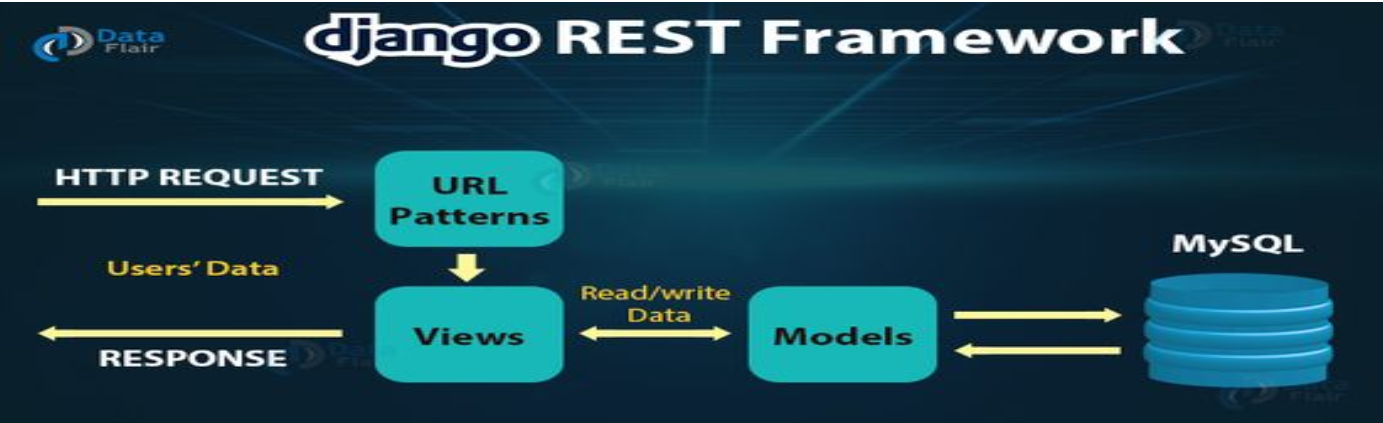
\includegraphics[scale=0.6]{django.png}}
  \caption{Modelo-Vista-Template Django}
\end{figure}

Cuando hacemos una consulta a la web, esta consulta accede al mapa de URLs, cada ruta está asociada a una vista, 
esa vista decide si necesita hacer una consulta a la base de datos, y, por tanto, irá a los modelos y después se 
mostrará la información a través de un template o directamente se muestra la información en un template.

\subsection{Lenguaje de programación}

Una vez elegido el Framework \textbf{Django}, como lenguaje de programación no nos queda otra que utilizar \textbf{Python} como lenguaje de programación.\\\\
\textbf{Python} es un lenguaje multipropósito, es entendible y simple, además de tener una curva de aprendizaje baja frente a otros lenguajes tan estrictos como \textbf{C}, 
tiene gran variedad de Frameworks, gran entorno de librerías y es multiplataforma.\\ \\

\section{Base de datos} \label{sec:base_datos}

\subsection{Tecnología}

Para elegir que gestor de base de datos utilizar en el proyecto primero debemos pensar en qué necesidades tenemos.
Las dos características principales que deben cumplir es que sea escalable y que funcione bien en ambientes de alto volumen 
de datos ya que la aplicación comenzará a funcionar con un número pequeño de productos alimenticios pero la idea es almacenar una gran cantidad de datos.\\ \\
Mis opciones eran \textbf{PostgreSQL} y \textbf{MongoDB}, aunque obviamente hay muchas más opciones, estas son las que conozco de haber trabajado con ellas y
más fácil me va a ser trabajar con ellas.\\ \\

En ese aspecto tanto \textbf{PostgreSQL} como \textbf{MongoDB} son buenas opciones ya que cumplen esas características.\\ \\

"\textbf{MongoDB} \cite{NoSQL} es una base de datos NoSQL potente que nos permitirá almacenar cualquier información que nuestra aplicación web necesite. Desde Python podemos acceder a la base de datos MongoDB usando el cliente Pymongo".

Por otro lado, \textbf{PostgreSQL} es una base de datos SQL también muy potente, con gran escalabilidad y con la que podremos almacenar cualquier información que necesitemos.\\

Ambas son muy buenas opciones para nuestro proyecto pero finalmente me he decidido por \textbf{PostgreSQL}, ya que para el despliegue \ref*{sec:despliegue} nos va a facilitar mucho las cosas
al tener un uso gratuito con \textbf{Heroku}.

\subsection{Configuración}

Una vez creado nuestro proyecto de Django, por defecto nos viene configurado para usar sqlite, pero configurarlo con PostgreSQL va a ser muy sencillo.
Simplemente tenemos que instalar la librería \textbf{psycopg2} y en el archivo settings crear una base de datos que tenga el motor de PostgreSQL en lugar de sqlite3.
Además, debemos indicarle un nombre, host, credenciales de usuario y contraseña y puerto (normalmente 5432).\\ \\

Una vez hecho esto debemos crear nuestros modelos de la base de datos.

\subsection{Modelos}

Para el diseño de las estructuras de datos y en este caso, los modelos, se va a seguir el \textbf{diseño guiado por el dominio} \cite{DDD} (domain-driven design o DDD).\\ \\

Es un serie de prácticas y terminologías que hacen que se cree una comunicación efectiva entre expertos del dominio, en este caso dietistas, nutricionistas o gente con 
grandes conocimientos acerca de la alimentación, y los desarrolladores.\\

\begin{figure}[H]
  \centering
  \noindent\makebox[\textwidth]{
    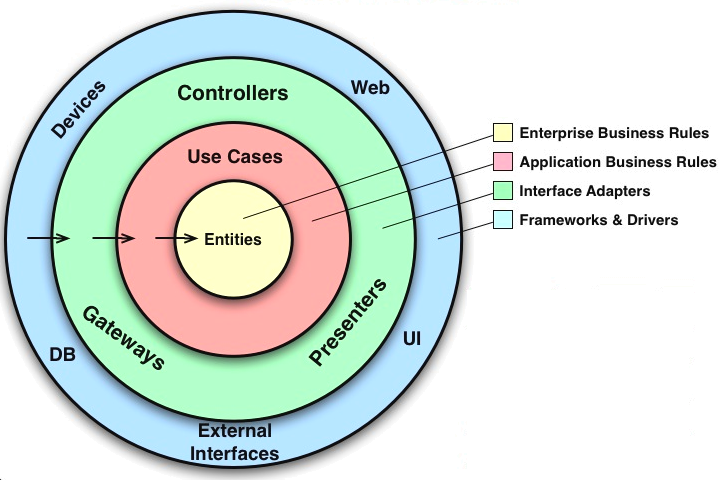
\includegraphics[scale=0.5]{domain-driven-design.png}}
  \caption{Domain-Driven-Design}
\end{figure}

Como se muestra en la figura, tenemos en el centro de todo las entidades o modelos. Una vez creados estos modelos, serán los propios usuarios y expertos en el modelo de negocio los que
mediante historias de usuario van a detallar las distintas funcionalidades que tendra el proyecto. A partir de ahí se crean los controladores (backend) y por último, tenemos el frontend,
en nuestro caso, una web.\\ \\

Esta manera de diseño hace que las capas más internas no sepan nada acerca de las externas, mientras que las externas se basan en las internas.

He creado los modelos producto, dieta y usuario, los modelos E/R se encuentran en el apéndice \ref*{apendiceB}\\
El modelo producto está formado por 23 datos que guardan información del producto como nombre, tienda, categoría.. y información nutricional como proteinas, hidratos, grasa...\\\\

\begin{figure}[H]
  \centering
  \noindent\makebox[\textwidth]{
    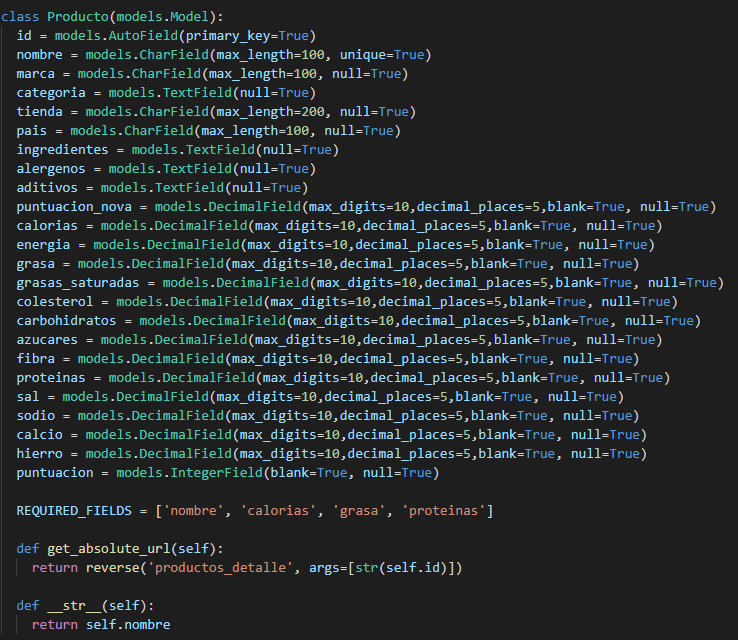
\includegraphics[scale=0.7]{productoModel.png}}
  \caption{Modelo producto}
\end{figure}

El modelo dieta está formado por un nombre, una descripción, una lista de productos y un usuario al que se le asigna.\\

\begin{figure}[H]
  \centering
  \noindent\makebox[\textwidth]{
    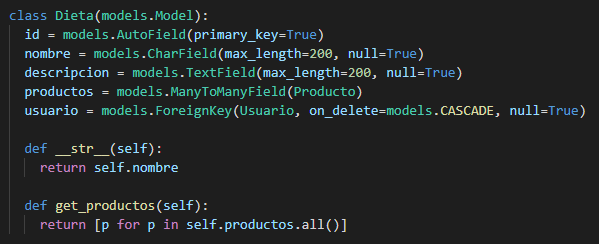
\includegraphics[scale=0.7]{dietaModel.png}}
  \caption{Modelo dieta}
\end{figure}

Para el modelo del usuario he utilizado la librería \textbf{django.contrib.auth.models} de Django, 
esta librería nos da toda la funcionalidad necesaria para crear usuarios, iniciar sesión y cerrarla. 
El problema es que sólo tiene los atributos username, password, email, nombre y apellidos.\\\\

Para solucionar esto he utilizado otra librería llamada \textbf{Base Abstract user} que te permite a partir 
de la librería anterior crear un modelo de usuario modificado con los atributos que nosotros queramos.\\

Para ello creamos el siguiente modelo de usuario, en el que tenemos atributos como peso, altura, edad, sexo y fecha de nacimiento.

\begin{figure}[H]
  \centering
  \noindent\makebox[\textwidth]{
    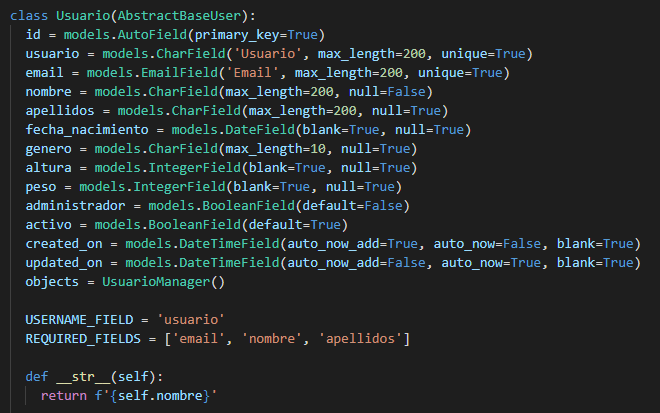
\includegraphics[scale=0.7]{usuarioModel.png}}
  \caption{Modelo usuario}
\end{figure}

Una vez tenemos el modelo de usuario simplemente en el settings indicamos dicho modelo y creamos las funciones 
para crear usuarios y súper usuarios.\\

\begin{figure}[H]
  \centering
  \noindent\makebox[\textwidth]{
    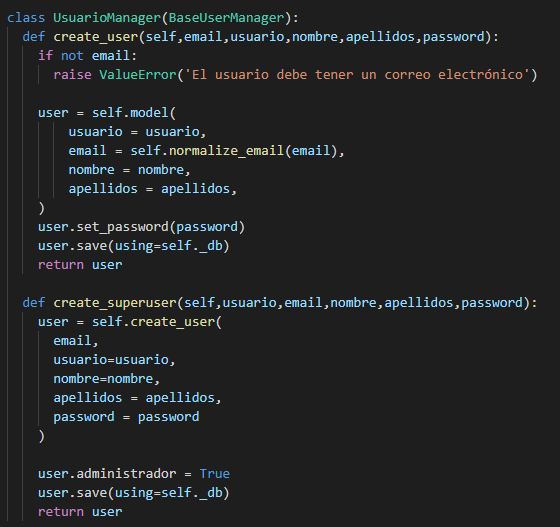
\includegraphics[scale=0.7]{usuarioManager.png}}
  \caption{Modelo usuario manager}
\end{figure}

\subsection{Datos}

Los datos han sido descargados de la web de \textbf{Open Food Facts}, como expliqué en la sección de estado del arte \ref{sec:estado_del_arte}.
Han sido utilizados porque es una gran cantidad de productos los que contiene esa base de datos y te permite descargarlos en diferentes formatos y, muy importante,
son de código abierto.\\ \\

En esta ocasión he obtenido los datos en formato CSV y para la limpieza de datos he utilizado \textbf{Excel}, sin embargo, la idea es automatizar esta tarea en un futuro
con \textbf{scripts de Python}, para ello podriamos utilizar la librería \textbf{Pandas}.

En cuanto a eliminar campos he hecho lo siguiente:
\begin{enumerate}
  \item He eliminado los productos cuyo nombre estuviera vacío.
  \item He eliminado valores que no fueran correctos:
  \begin{itemize}
    \item Valores calóricos que eran exageradamente grandes.
    \item Valores calóricos que eran exageradamente pequeños.
  \end{itemize}
  \item Campos que contenían caracteres especiales
\end{enumerate}

Una vez eliminados esos valores, he filtrado por productos que son procedentes de España ya que por el momento me eran suficientes.
Cuando el proyecto vaya avanzando en el desarrollo se irán incluyendo productos de otros países, pero ahora mismo la base de datos era
 demasiado grande para las herramientas que he utilizado en el despliegue \ref{sec:despliegue}.\\

\section{Backend} \label{sec:backend}

Voy a explicar la funcionalidad de la aplicación, así como las funciones más interesantes y las bibliotecas o paquetes utilizados para ello, podemos consultar el manual de usuario en el apéndice C \ref*{apendiceC}. \\ \\

Para el modelo de usuario podemos registrarnos y crear nuestro perfil, a demás de consultarlo, modificarlo y eliminarlo.
Si iniciamos sesión podemos consultar el lsitado total de productos que hay en la web así como buscar el que queramos, consultarlo en detalle y
modificarlo y eliminarlo si somos administradores o pertenecemos al grupo de dietistas.\\ \\

Para el paginador de la vista listado de productos he utilizado \textbf{django.core.paginator} de Django. Este paquete nos permite crear 
un paginador muy fácil simplemente llamamos a la función Paginador pasándole dos parámetros, un listado con los objetos que 
queramos mostrar y el número en el que queremos dividirlo (productos a mostrar por página). \\ \\

Para la generación de dietas en un principio la idea era utilizar un algoritmo de la mochila con el que a partir de un formulario obtuvieramos los datos del solicitante
como el peso, altura, sexo y objetivos, y en base a eso obtener unas cantidades de proteinas, grasas, etc que tuvieramos que alcanzar.\\ \\

El algoritmo trabajaría con esos parámetros y generaría una dieta que alcanzara esas cantidades de nutrientes específicos, pero finalmente esa idea fué descartada por dos motivos.\\\\

Primero por eficiencia, ya que queremos tener una gran cantidad de productos y un algoritmo así tardaría una gran cantidad de tiempo en hacer esos cálculos, además el otro motivo es 
porque la gente con conocimientos sobre nutrición, como dietistas y culturistas, a la que he consultado me han comentado lo mismo, que no se puede conseguir una dieta optimizada con esos 
parámetros ya que es todo mucho más complicado, es decir, de esa manera obtendriamos una dieta optimizada con la que ganar peso para una persona y esa misma dieta para otra persona con 
las mismas características no obtendrían los mismos resultados. Esto es debido a nuestros metabolismos y es muy complicado calcularlo.\\\\

Ante esto, entre yo y estas personas pensamos que lo mejor era poder solicitar estas dietas pero que en vez de generarlas con un algoritmo de la mochila, estuvieran ya creadas previamente
y sólo se tendría que elegir una en función de los objetivos y características del usuario. Una vez obtenida la dieta, para optimizarla vamos a desarrollar una función con la que 
obtengamos productos que sean similares entre sí, nutricionalmente hablando.\\\\

Esto haría que nosotros podamos ir probando nuevos productos e incluirlos en nuestras dietas en función de qué nos va mejor o peor, además nos da la opción de encontrar productos más asequibles de precio si así los quisieramos y que se ajustaran más a nuestros gustos.

\section{Frontend} \label{sec:frontend}

Para el Frontend del proyecto a desarrollar vamos a realizar una \textbf{aplicación web} ya que para los dietistas les va a ser mucho más cómodo
crear sus dietas y consultar información que, desde una aplicación móvil, y para los demás usuarios pueden consultarlo desde otros dispositivos, si así lo quisieran, 
debido a que el diseño va a ser adaptable para todo tipo de dispositivos.

Para ello, voy a utilizar \textbf{Bootstrap} \cite{bootstrap} ya que nos permite diseñar sitios webs de manera sencilla,
es de código abierto, es compatible con todos los navegadores y sus diseños son adaptables por lo que funcionan en todos los dispositivos,
además, es muy completo y presenta una gran variedad de componentes muy útiles como modales, tablas, alertas, botones...\\ \\

La idea de diseño de la web ha sido cogida de la plantilla de \textbf{AdminLTE} \cite{adminlte}. Esta plantilla es de código abierto y 
además, incluye muchos componentes útiles.

Para los iconos he utilizado la web open source \textbf{FontAwesome} \cite{iconos} que nos 
ofrece una gran cantidad de iconos gratis además de dar la capacidad de elegir el tamaño de ellos.

\subsection{Formularios}

Otra parte importante serán los formularios, con estos podremos crear y modificar los modelos creados anteriormente.

\begin{figure}[H]
  \centering
  \noindent\makebox[\textwidth]{
    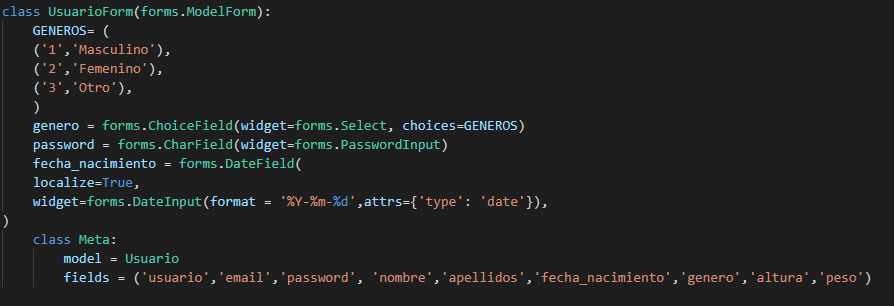
\includegraphics[scale=0.7]{usuarioForm.png}}
  \caption{Formulario de usuario}
\end{figure}

\begin{figure}[H]
  \centering
  \noindent\makebox[\textwidth]{
    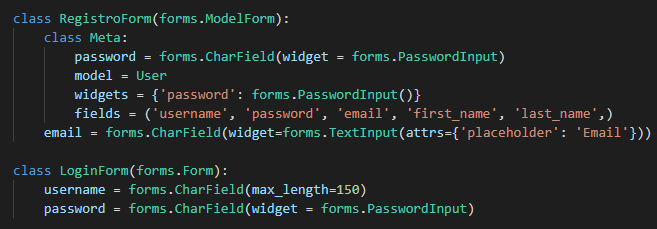
\includegraphics[scale=0.7]{registroLoginForm.png}}
  \caption{Formularios de registro y login}
\end{figure}

\newpage
\section{Tests} \label{sec:tests}

Los tests son una parte muy importante del proyecto ya que sin ellos no sabes si has llevado a cabo las historias de usuario o no, por tanto, 
podemos decir que es la forma de asegurar la calidad del software. \\ \\

Para los tests emplearé la biblioteca \textbf{TestCase}. Es la más común en Django para la creación de test.\\
Esta biblioteca es una extensión de SimpleTestCase, pero esta sólo vale si no utilizas una base de datos 
en tu aplicación.\\

Para cada una de las funcionalidades de la web vamos a crear un test y con ella cerraremos la issue corespondiente.
Este sería un ejemplo en la que testeamos las funciones de crear y modificar un producto.

\begin{figure}[H]
  \centering
  \noindent\makebox[\textwidth]{
    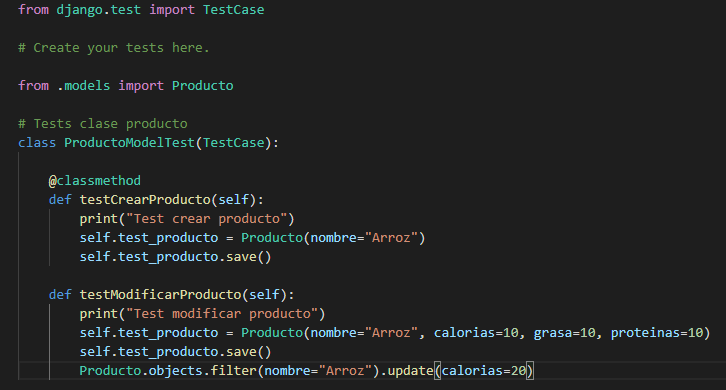
\includegraphics[scale=0.7]{test.png}}
  \caption{Test}
\end{figure}

\section{Despliegue} \label{sec:despliegue}

\subsection{Plataforma}

Por último, quedaría desplegar la aplicación, para ello voy a utilizar \textbf{Heroku}.\\

Ante las necesidades del proyecto de encontrar una plataforma de despliegue en la nube que fuera fácil de usar, pudiera actualizarse de manera automática, fuera gratuita y permitiese el lenguaje Python decidí utilizar Heroku ya que cumplía todas estas necesidades. 

\textbf{Heroku} es una plataforma en la nube que nos permite desplegar aplicaciones web en cualquier lenguaje de programación.
Además, es muy sencillo, sólo tenemos que conectar nuestro repositorio de GitHub en el que tengamos el proyecto que queremos desplegar,
podemos configurarlo para que con cada commit se haga el despliegue automáticamente y además es gratuito. Otras alternativas a Heroku 
eran Firebase y Azure.

\subsection{Librerías}

La primera librería que tenemos que instalar es \textbf{Gunicorn}. Esta librería es un servidor HTTP para Unix, sin ella nos sería imposible realizar el despliegue de nuestra aplicación.
Como en este proyecto estamos trabajando con base de datos PostgreSQL, necesitamos instalar la librería \textbf{psycopg2}. Esta librería es un adaptador a dicha base de datos para el lenguaje Python.\\\\
Heroku por defecto no permite los archivos estáticos, para solucionar este problema he incluido la librería \textbf{whitenoise}.\\
Esta librería nos permite cargar todos los archivos estáticos y se configura muy fácil, simplemente tenemos que instalarlo y en
el fichero settings.py de la aplicación incluimos el middleware y las rutas de dichos archivos que queremos cargar.\\\\
Por último, necesitamos dos librerías más, una de ellas es \textbf{dj-database-url}. Esta librería realiza la conexión entre nuestro proyecto y el gestor de base de datos de Heroku.\\
Y la otra librería es \textbf{python-decouple} para usar variables de entorno en Heroku, así evitamos poner tokens y contraseñas a la vista de todos en nuestro proyecto. \\

Por tanto, el archivo requirements.txt quedaría así:
\begin{figure}[H]
  \centering
  \noindent\makebox[\textwidth]{
    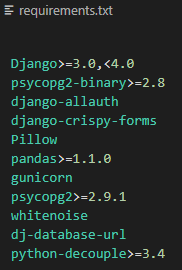
\includegraphics[scale=1]{requirements.png}}
  \caption{Archivo requirements.txt}
\end{figure}


\subsection{Configuración}

Para configurar el despliegue en Heroku como he explicado anteriormente debemos registrarnos en la web y conectar el repositorio de Github del proyecto.
Una vez hecho esto nos vamos al archivo settings.py del proyecto y hacemos lo siguiente:\\
Importamos las librerías, ponemos debug a false e incluimos en allowed\_hosts la url de despliegue o simplemente ponemos un asterisco y así acepta todas las urls.

\begin{figure}[H]
  \centering
  \noindent\makebox[\textwidth]{
    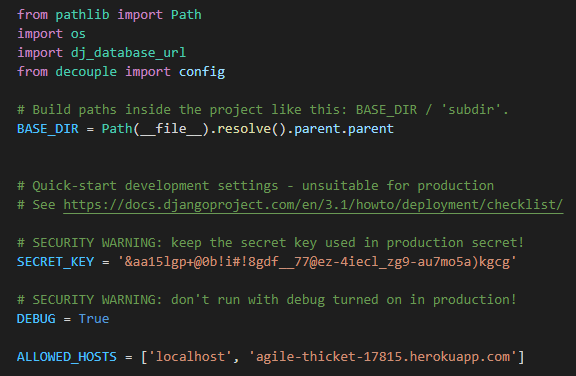
\includegraphics[scale=0.8]{settings1.png}}
  \caption{Configuración despliegue}
\end{figure}

Añadimos el middleware de whitenoise.

\begin{figure}[H]
  \centering
  \noindent\makebox[\textwidth]{
    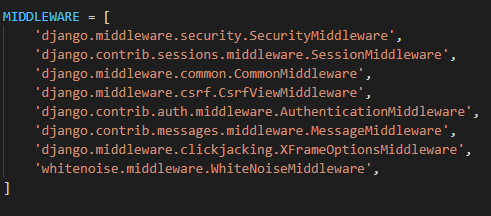
\includegraphics[scale=1]{settings2.png}}
  \caption{Configuración despliegue middleware}
\end{figure}

Indicamos la base de datos.

\begin{figure}[H]
  \centering
  \noindent\makebox[\textwidth]{
    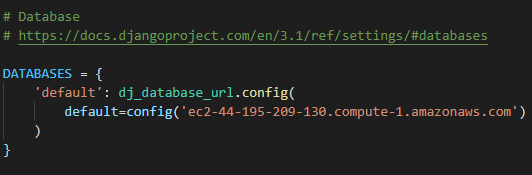
\includegraphics[scale=1]{settings3.png}}
  \caption{Configuración despliegue base de datos}
\end{figure}

Añadimos esta línea para que whitenoise cargue los archivos estáticos.

\begin{figure}[H]
  \centering
  \noindent\makebox[\textwidth]{
    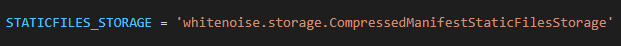
\includegraphics[scale=1]{settings4.png}}
  \caption{Configuración despliegue archivos estáticos}
\end{figure}

Ya tendríamos configurado todo. Simplemente tenemos que esperar a que se haga el despliegue si hemos configurado que se haga automáticamente con cada commit o desplegarlo nosotros desde la web.\\\\

Otra opción sería hacerlo desde local.
Nos conectamos a nuestra cuenta de Heroku con Heroku login, creamos una app de heroku con heroku create y hacemos un push desde nuestro repositorio local con:
\begin{lstlisting}
git push --prefix app keroku master
\end{lstlisting}

Conectamos nuestra base de datos con nuestra app con el siguiente comando:
\begin{lstlisting}
heroku pg:psql <nombre_bd_heroku> --app <nombre_app_heroku>
\end{lstlisting}

Ahora sólo quedaría hacer un migrate de la base de datos con:
\begin{lstlisting}
heroku run python manage.py migrate
\end{lstlisting}

Incluimos nuestros archivos sql con nuestros datos de la base de datos.
\begin{lstlisting}
heroku pg:psql --app <nombre_app> < <archivo.sql>
\end{lstlisting}
Y abrimos la aplicación con heroku open.\\\\

Para probar la aplicación aquí dejo el enlace:

\url{https://organize-udiet.herokuapp.com/}

\section{Presupuesto} \label{sec:coste}

\subsection{Planificación de costes}

En este apartado se va a realizar una estimación de costes del proyecto, ya que en todo proyecto de ingeniería los costes tanto de implementación como de ejecución son muy importantes.\\

Los factores a tener en cuenta para esta estimación van a ser:

\begin{enumerate}
  \item Duración del proyecto
  \item Sueldo del programador
  \item Plataforma de despliegue
\end{enumerate}

La duración del proyecto ha sido de unos 6 meses.\\

El sueldo medio de un programador \cite{sueldo} de mis carácteristicas (recien terminado el Grado de Ingeniería Informática y sin especializar en un lenguaje concreto) es de unos \textbf{20000\euro}.\\
Esto se traduce en unos \textbf{55\euro} al día, que trabajando a jornada de 8 horas serían unos \textbf{6,8\euro} la hora.\\

Por tanto, de los 210 días (7 meses) que ha durado el proyecto, a unas 3 horas de media trabajadas cada día serían 630 horas, que multiplicadas por el sueldo anteriormente mencionado sería un total de \textbf{4284\euro}.

En principio este sería el coste de desarrollo, a partir de ahí tenemos que pagar la plataforma de despliegue.\\ \\
Si elegimos \textbf{Azure} \cite{azure} que es una de las plataformas más utilizadas, un servidor con 4 núcleos, 7GB de RAM y 1000GB de almacenamiento nos costará \textbf{200\euro} cada mes que queramos tener la aplicación desplegada.\\
